\section{Converge SPA}
Grænsefladen til Converge-SPA er i form af et website, og bruger et dynamisk frontend bibliotek React til at tilbyde en Desktop lignende brugervenlighed. Normalt er websider statiske og vil ikke kunne reagere på brugerens interaktion uden at skulle genindlæse siden. React gør at det html hjemmesiden er bygget på kan opdateres igennem DOM-api \cite[Dom-API]{converge-terms}. Derfor skrives hele Converge-SPA i React. 

Selve grænsefladen blev designet i Figma \cite[Figma]{converge-terms}, før udviklingen begyndte, dette var for at tilbyde hurtige iterationer over hvilken funktionalitet der var vigtigt.

Converge-SPA består af et hierarki af sider indeholdende de forskellige funktioner. På figur \ref{fig:mindmap} beskrives de forskellige muligheder for brugerens navigation.

\begin{figure}[H]
    \centering
  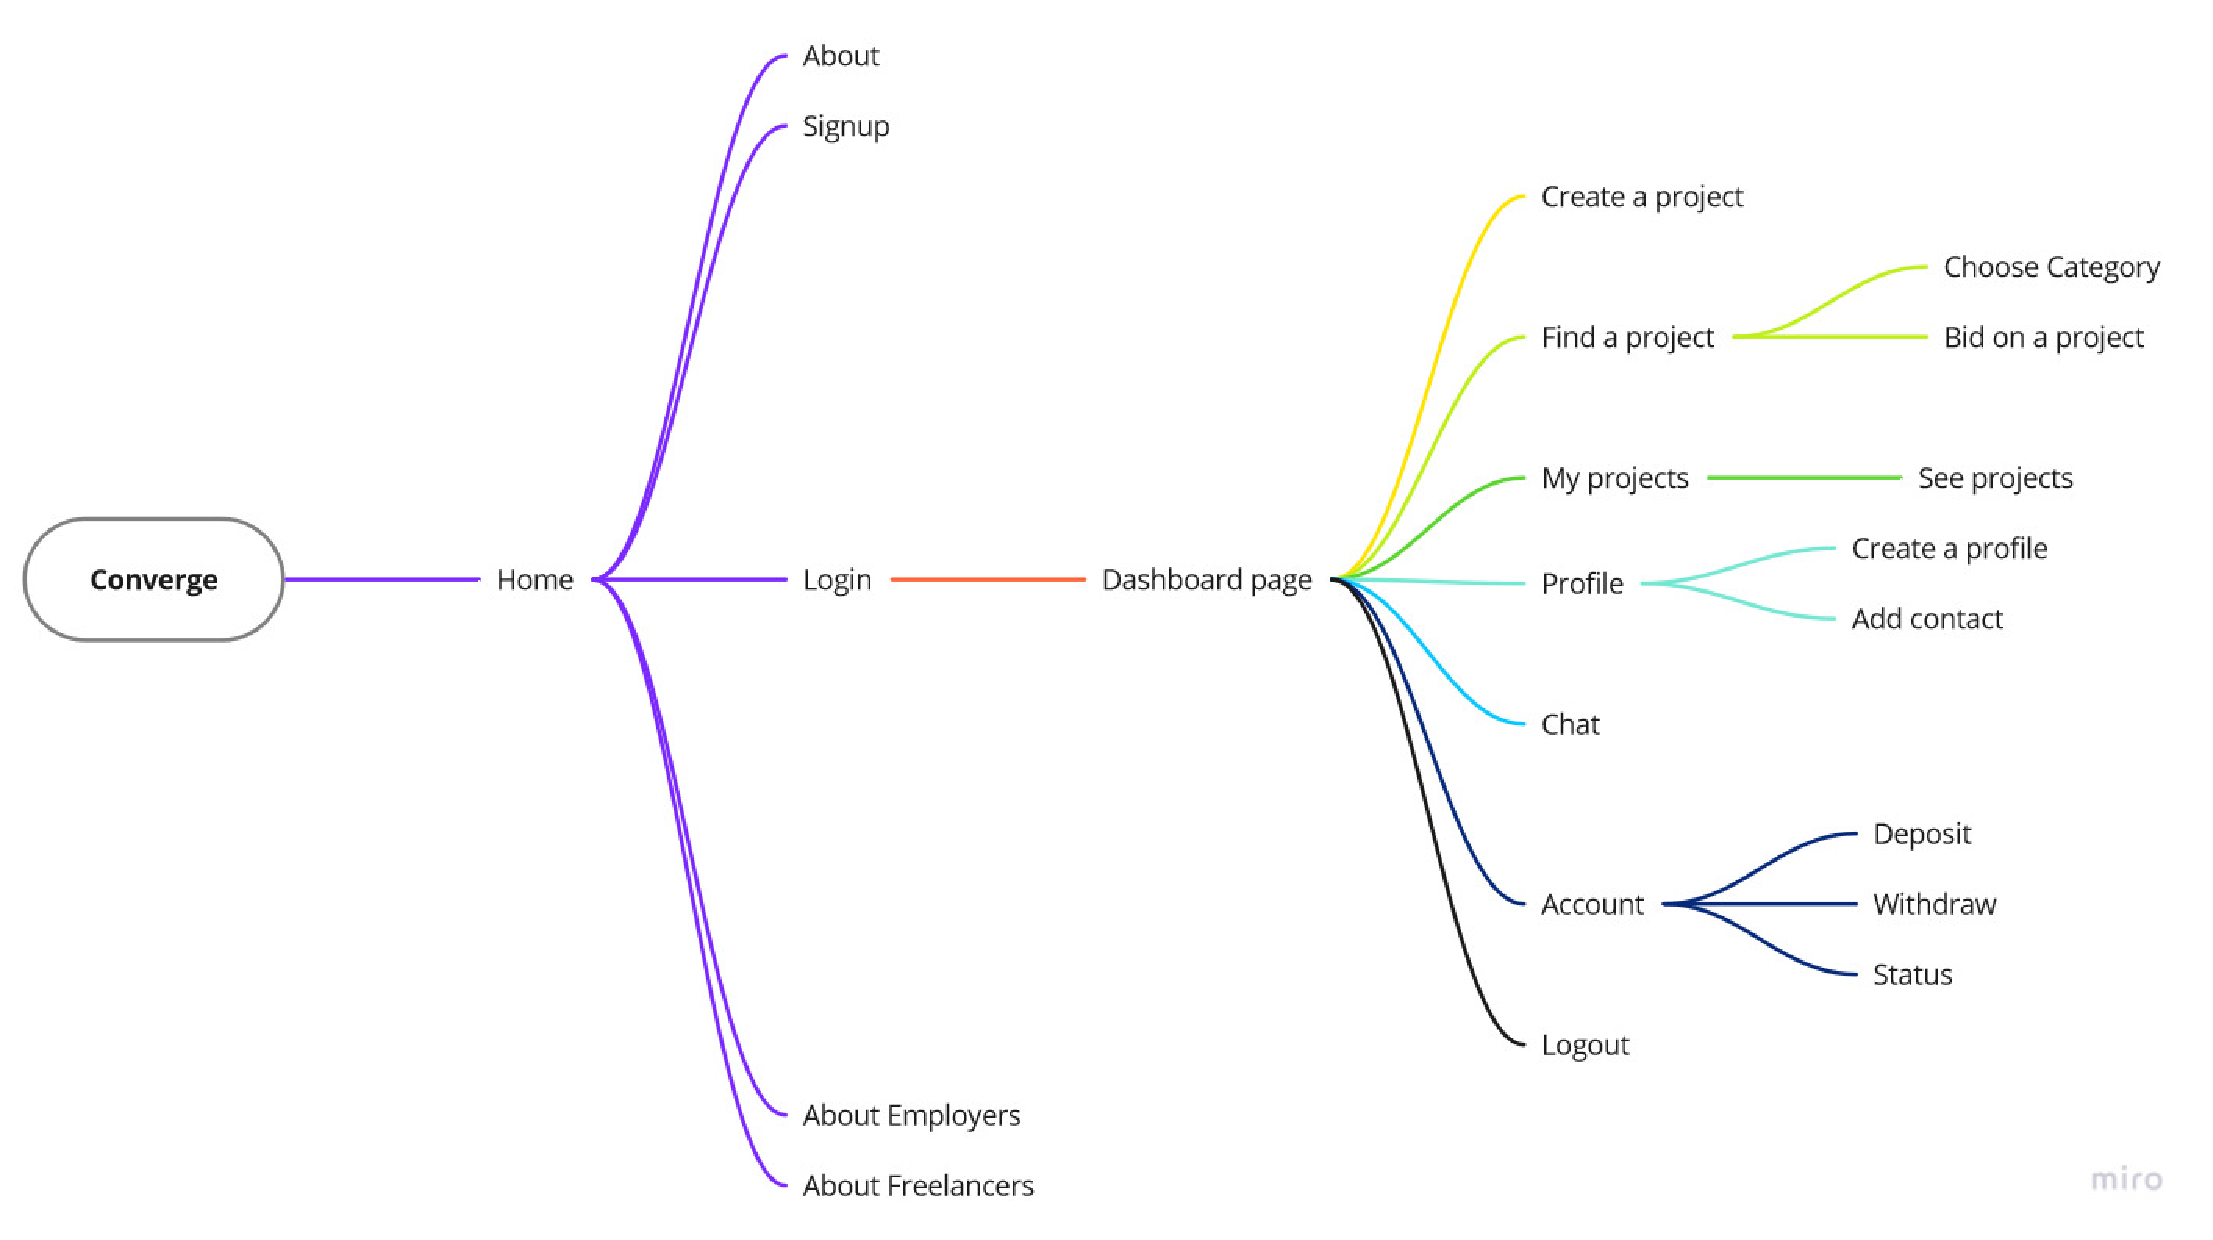
\includegraphics[width=0.8\textwidth]{Billeder/Converge-Mind-Map.pdf}
  \caption{Viser mind map over de forskellige \emph{pages}}
  \label{fig:mindmap}
  \end{figure}

Hver side er tilpasset til at skalere til en fuld desktop, en tablet eller en smartphone. Dette er for at tilbyde en glidende oplevelse fra de forskellige enheder. Selve designet følger et mørkt tema, med kontrast af hvidt og blåt til at vise Converge’s personlighed og karakter. Sammen med Material standarden fra Google, viser Converge et stilrent design, genkendeligt fra mange andre produkter på internettet, som Gmail, Facebook osv. Dog med dets egen kvalitet og karakter.

Nedenfor ses eksempel på en af mange Converge applikationens sider.

\begin{figure}[H]
    \centering
  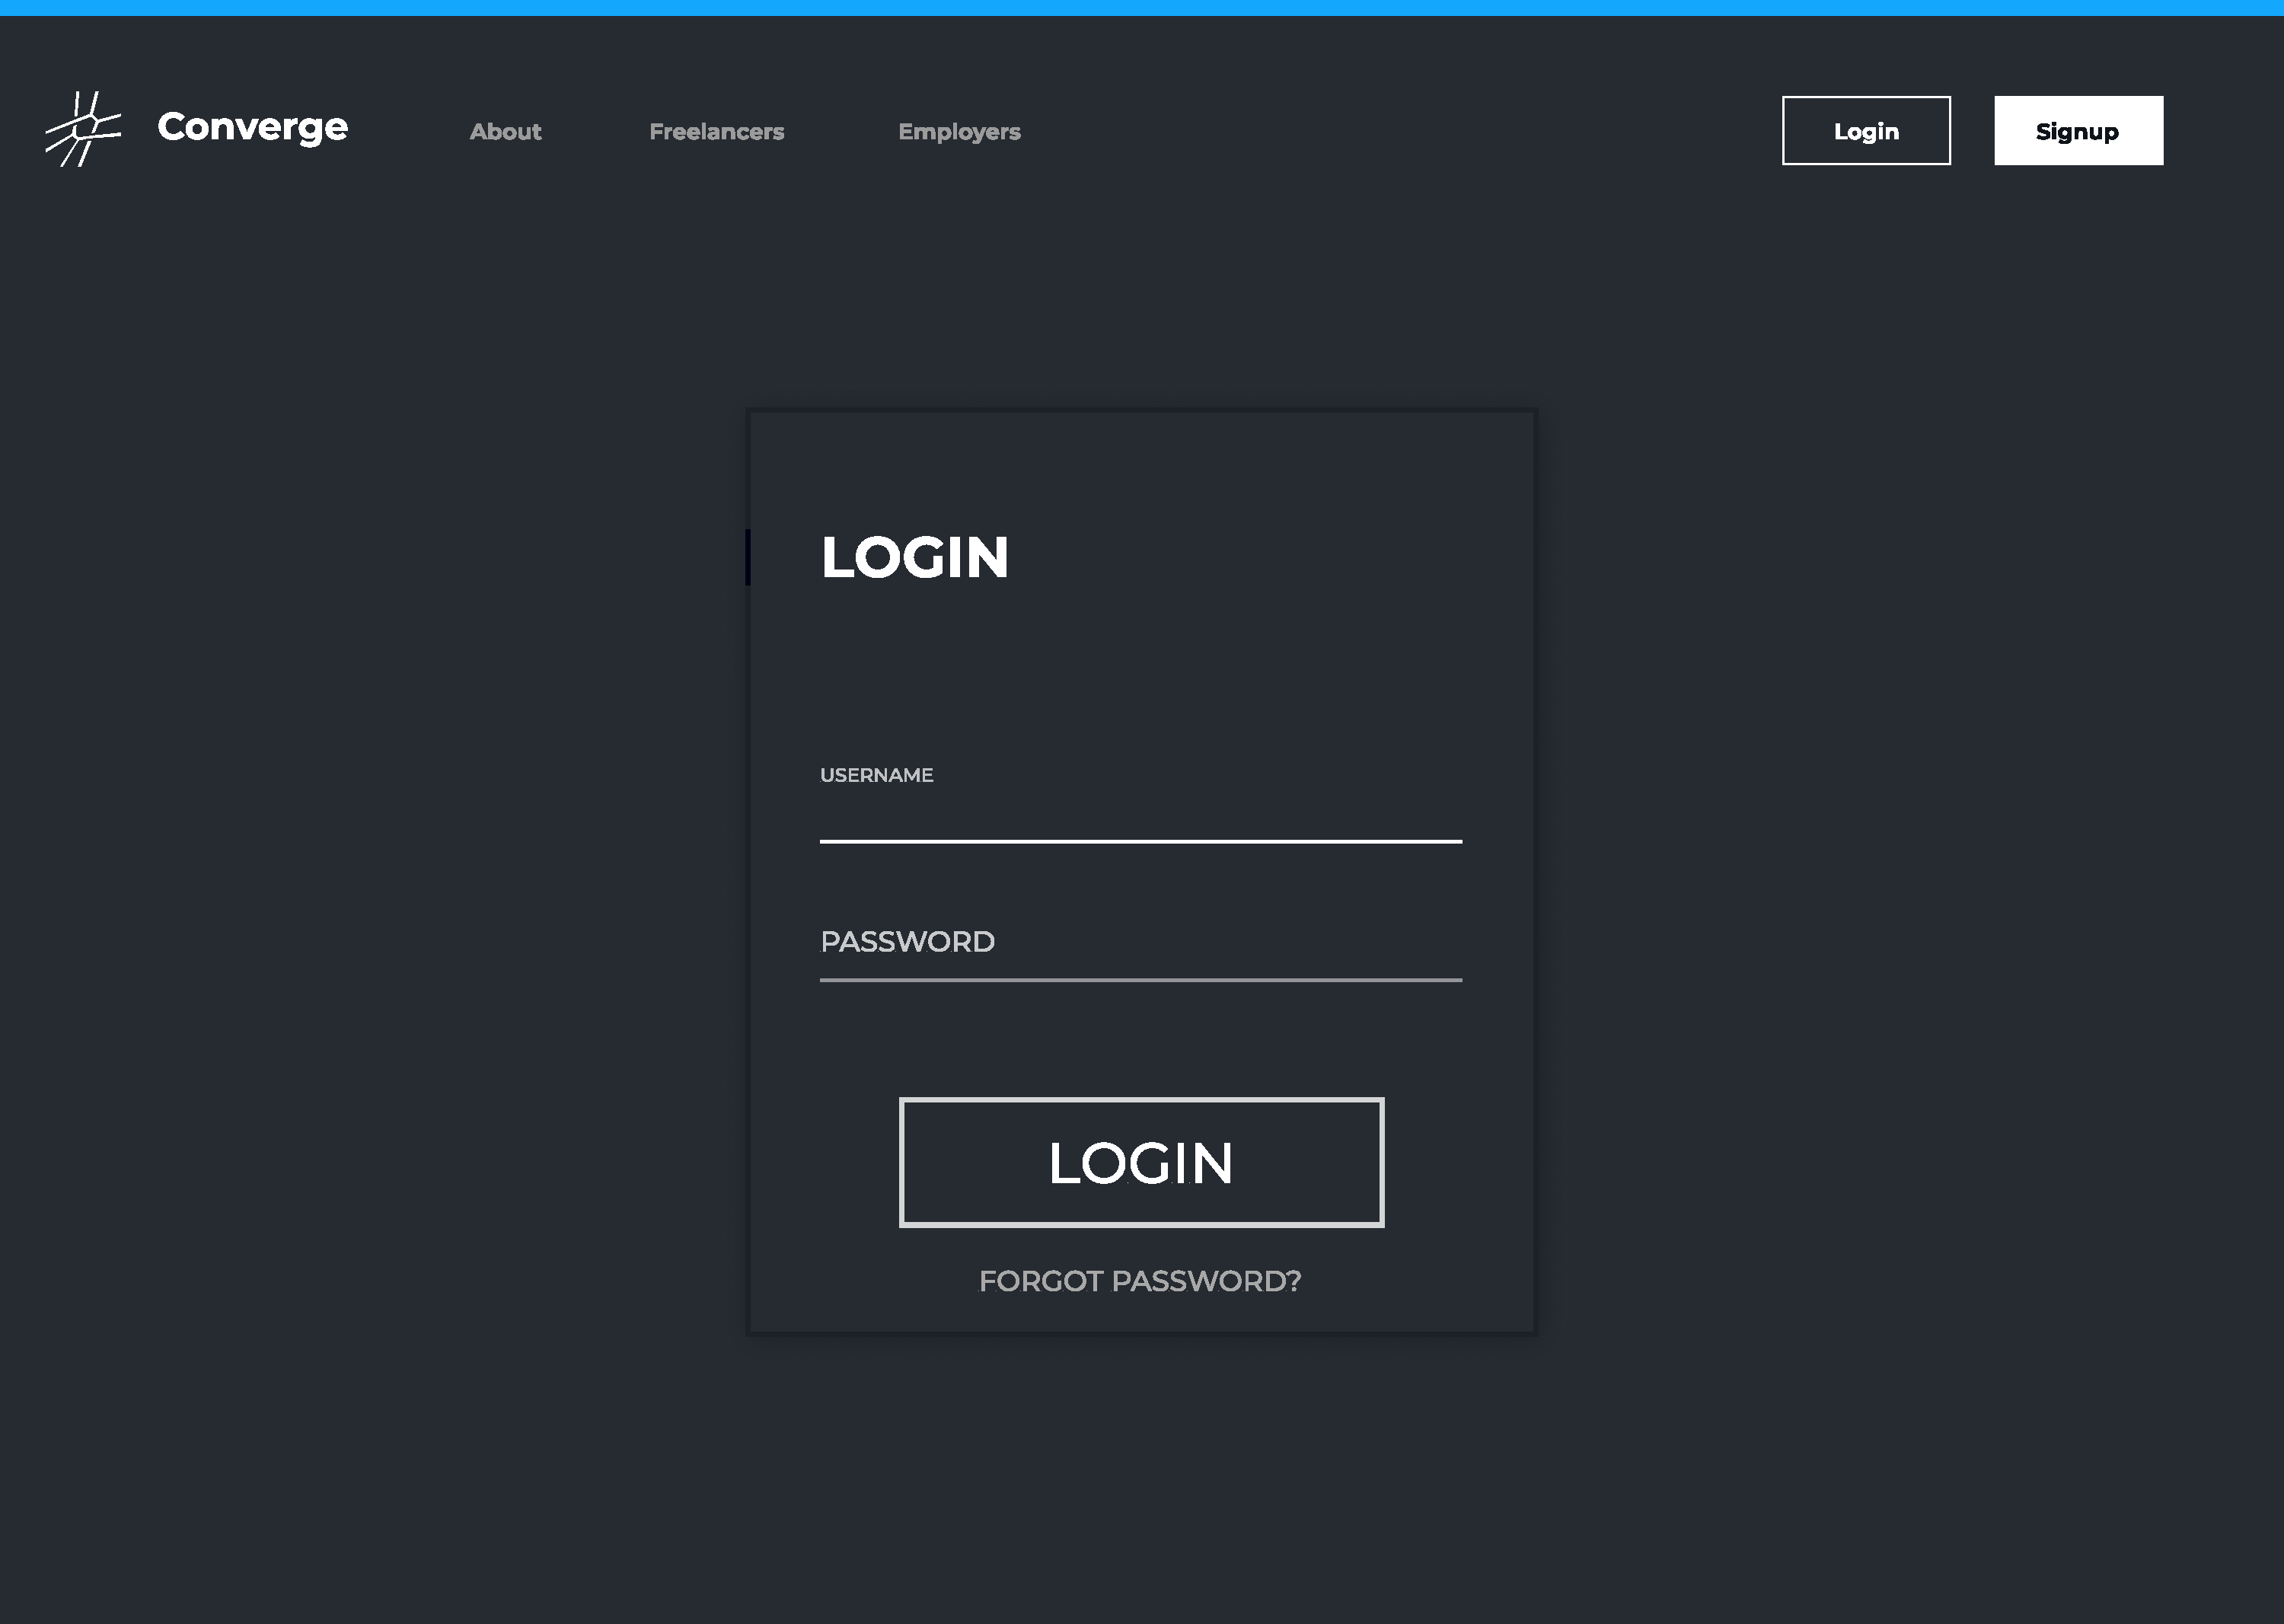
\includegraphics[width=0.8\textwidth]{Billeder/Login.pdf}
  \caption{Viser Login siden på Converge platformen}
  \label{fig:login}
  \end{figure}

Figur \ref{fig:login} viser login siden og her har brugeren muglighed for at kunne login med et valid login, som er
email og password.

\begin{figure}[H]
    \centering
  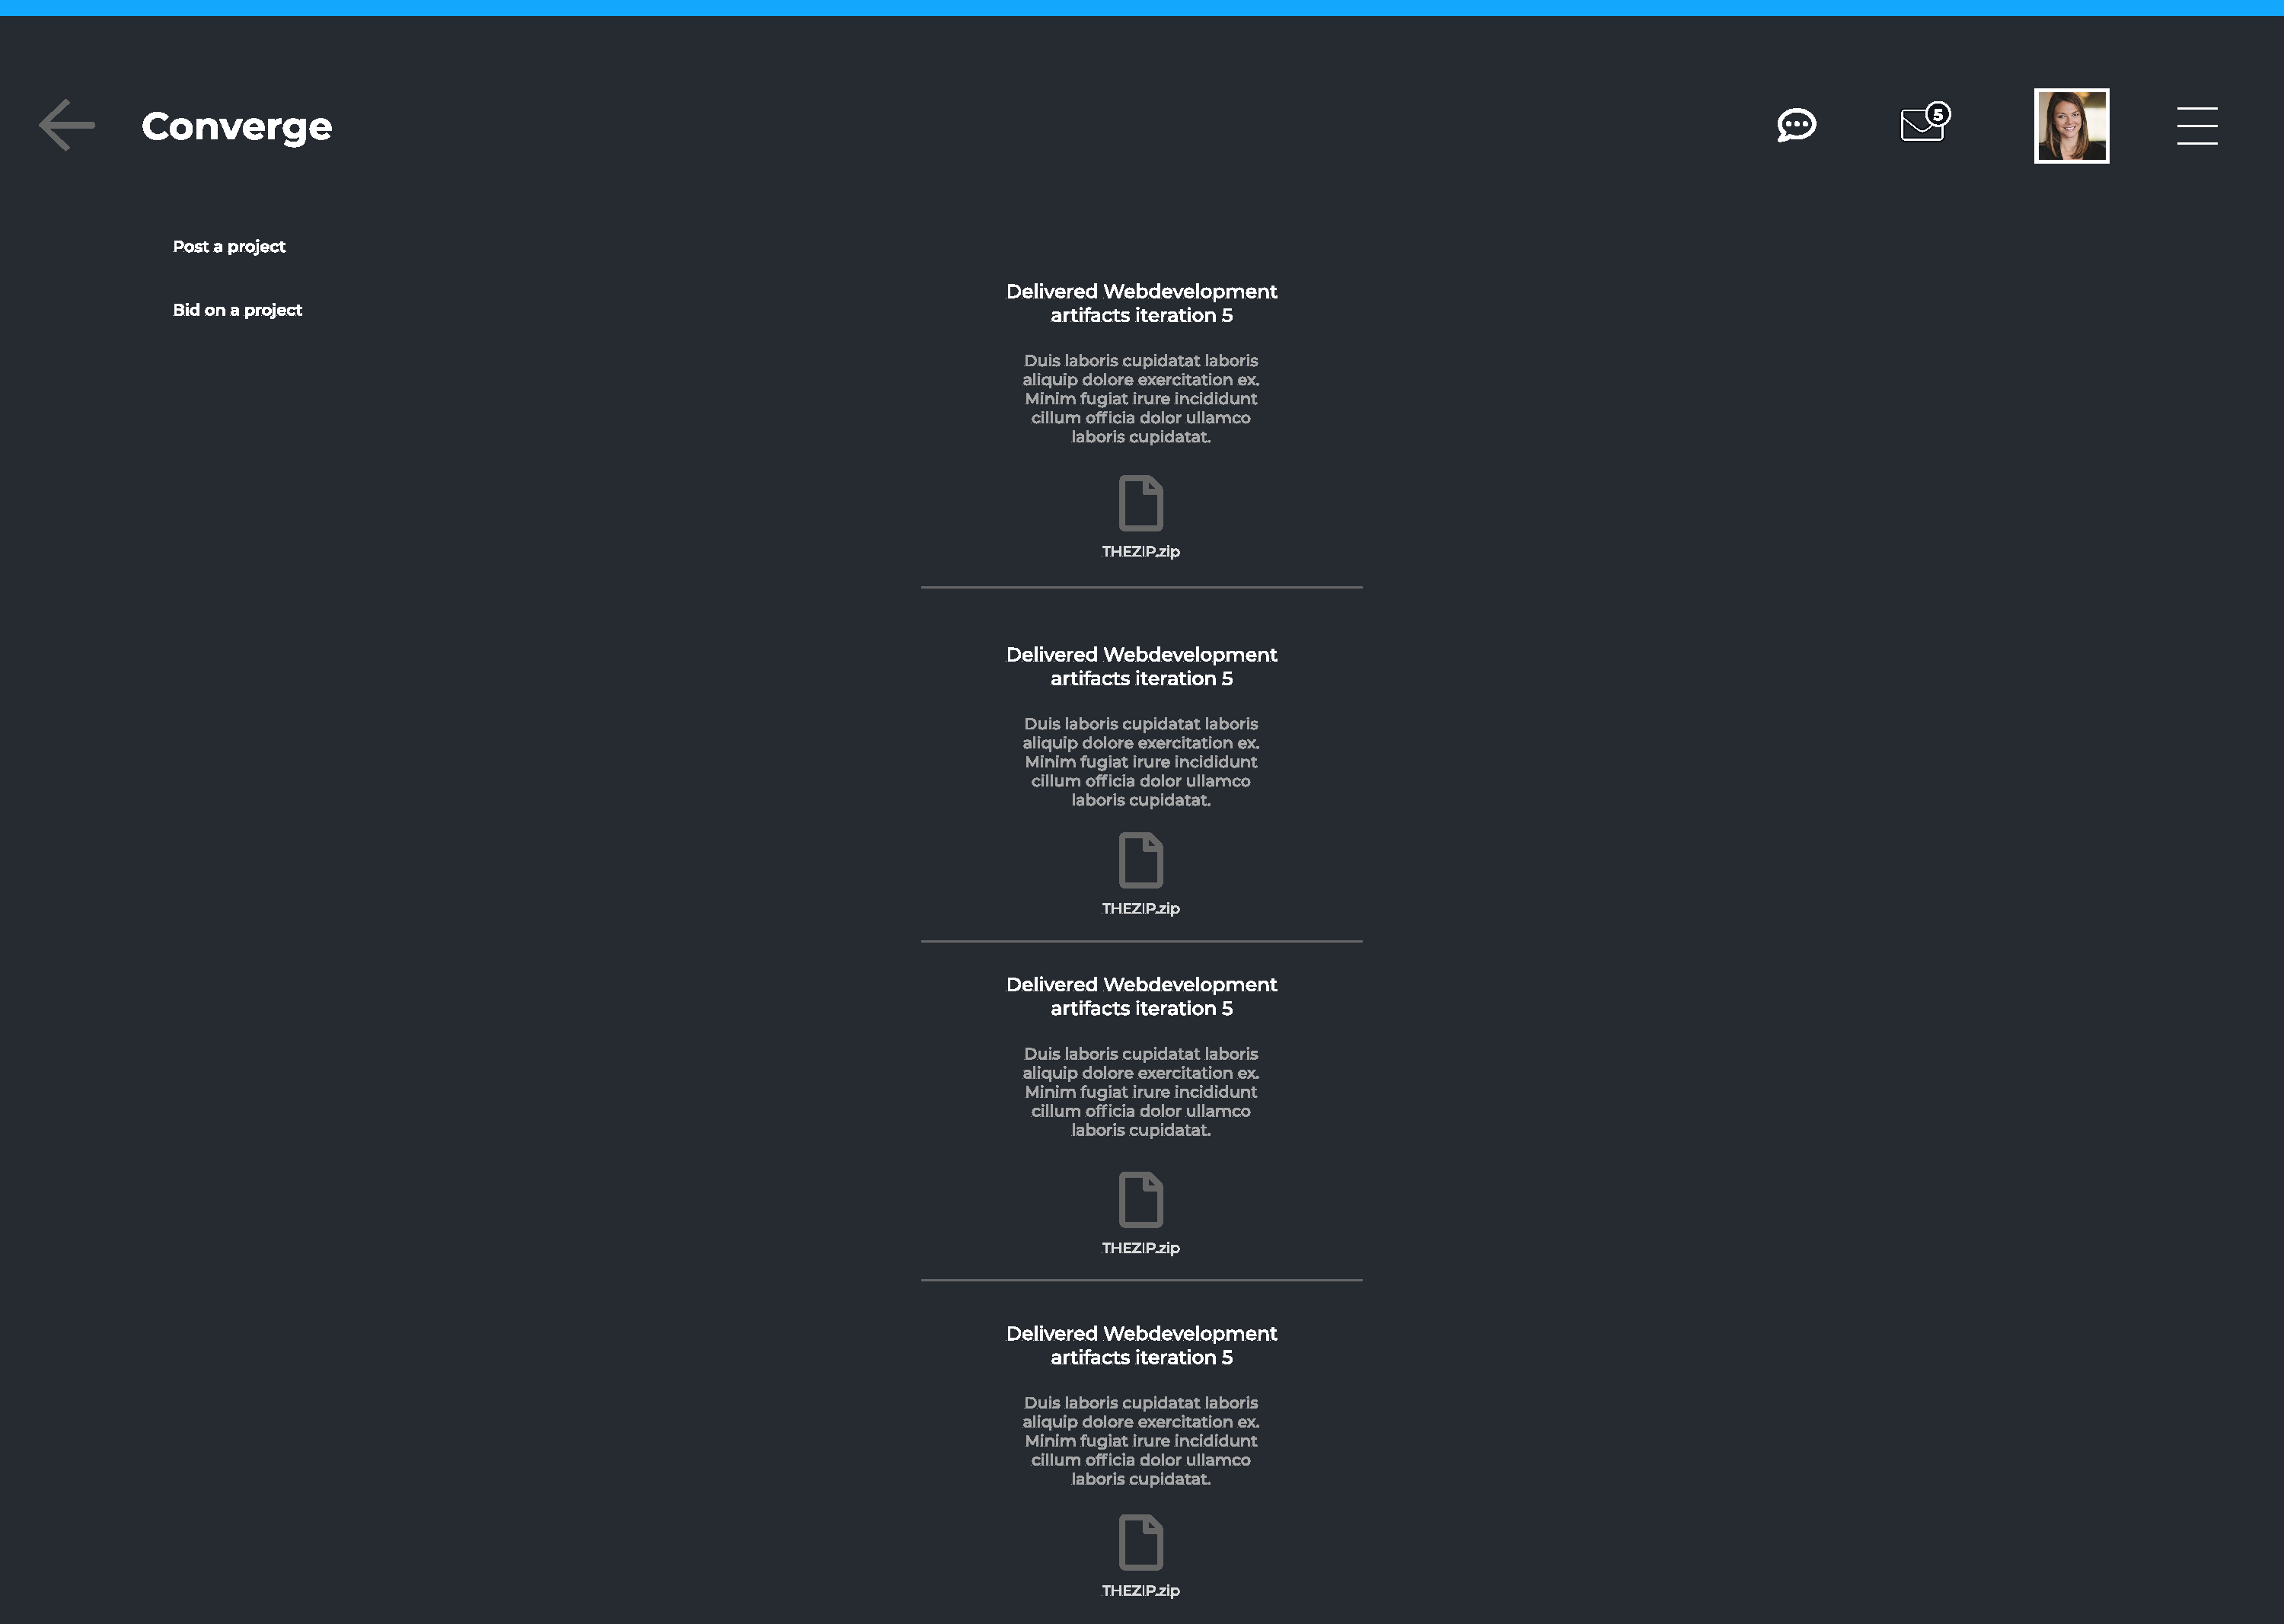
\includegraphics[width=0.8\textwidth]{Billeder/Dashboard.pdf}
  \caption{Viser dashboard siden på Converge platformen}
  \label{fig:dashboard}
  \end{figure}

Figur \ref{fig:dashboard} viser når man er logget ind, så bliver dashboard siden vist. Her kan
brugeren fortage sig forskellige handlinger. 

Der kan ses flere sider af Converge SPA i dokumentation \cite{system-interface}.